\chapter{Pruebas}

\section{Pruebas unitarias}

\begin{figure}[!ht]
	\begin{center}
		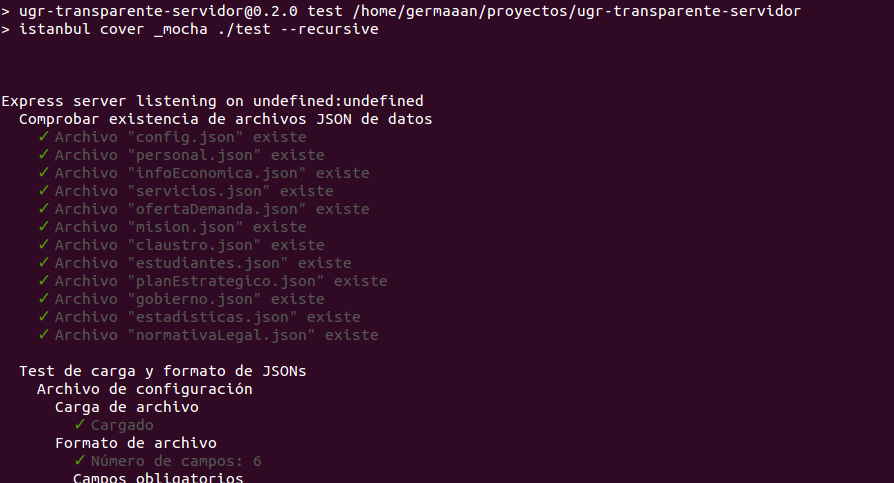
\includegraphics[width=1\textwidth]{../images/tests_unitarios_01.png}
		\caption{}
		\label{fig:tests_unitarios_01}
	\end{center}
\end{figure}

\begin{figure}[!ht]
	\begin{center}
		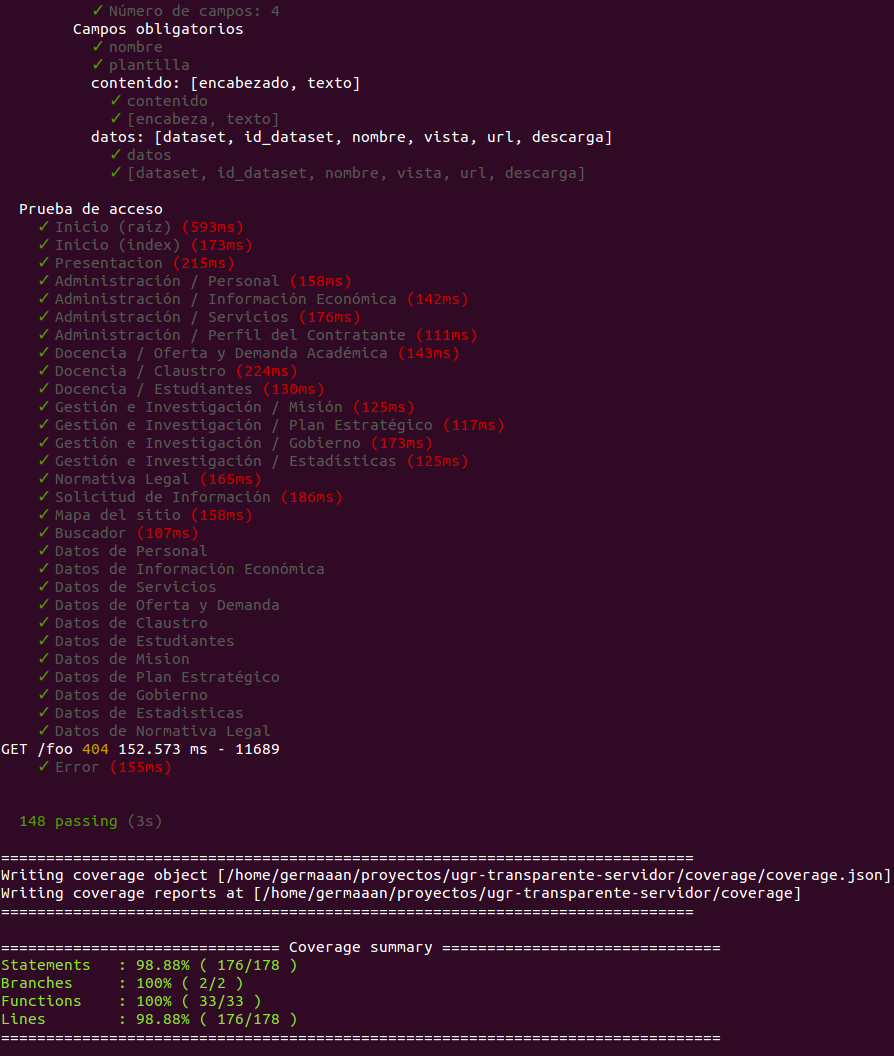
\includegraphics[width=1\textwidth]{../images/tests_unitarios_02.png}
		\caption{}
		\label{fig:tests_unitarios_02}
	\end{center}
\end{figure}

\section{Prueba de cobertura}

\begin{figure}[!ht]
	\begin{center}
		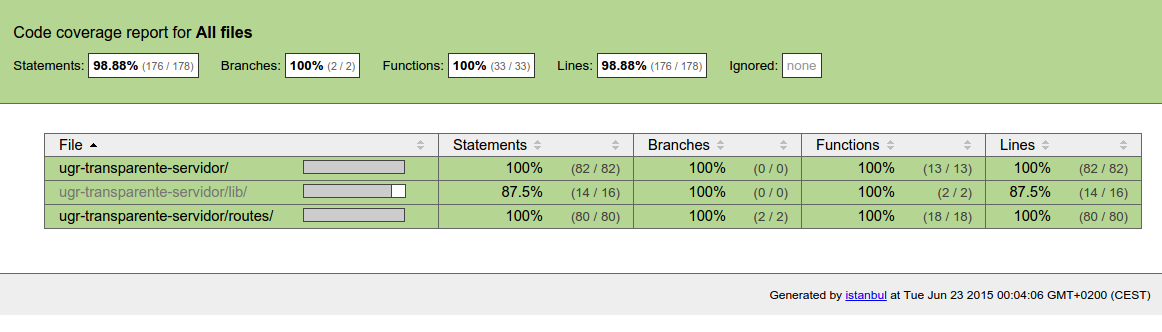
\includegraphics[width=1\textwidth]{../images/test_cobertura_01.png}
		\caption{}
		\label{fig:test_cobertura_01}
	\end{center}
\end{figure}

\begin{figure}[!ht]
	\begin{center}
		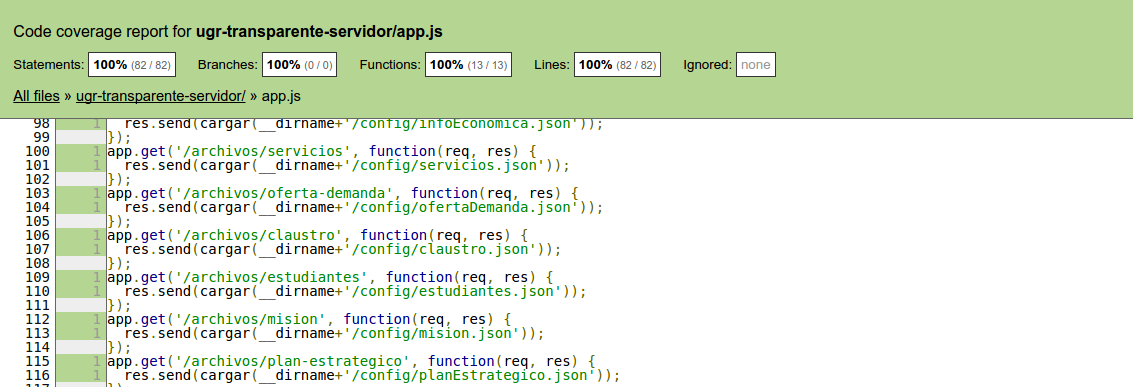
\includegraphics[width=1\textwidth]{../images/test_cobertura_02.png}
		\caption{}
		\label{fig:test_cobertura_02}
	\end{center}
\end{figure}

\begin{figure}[!ht]
	\begin{center}
		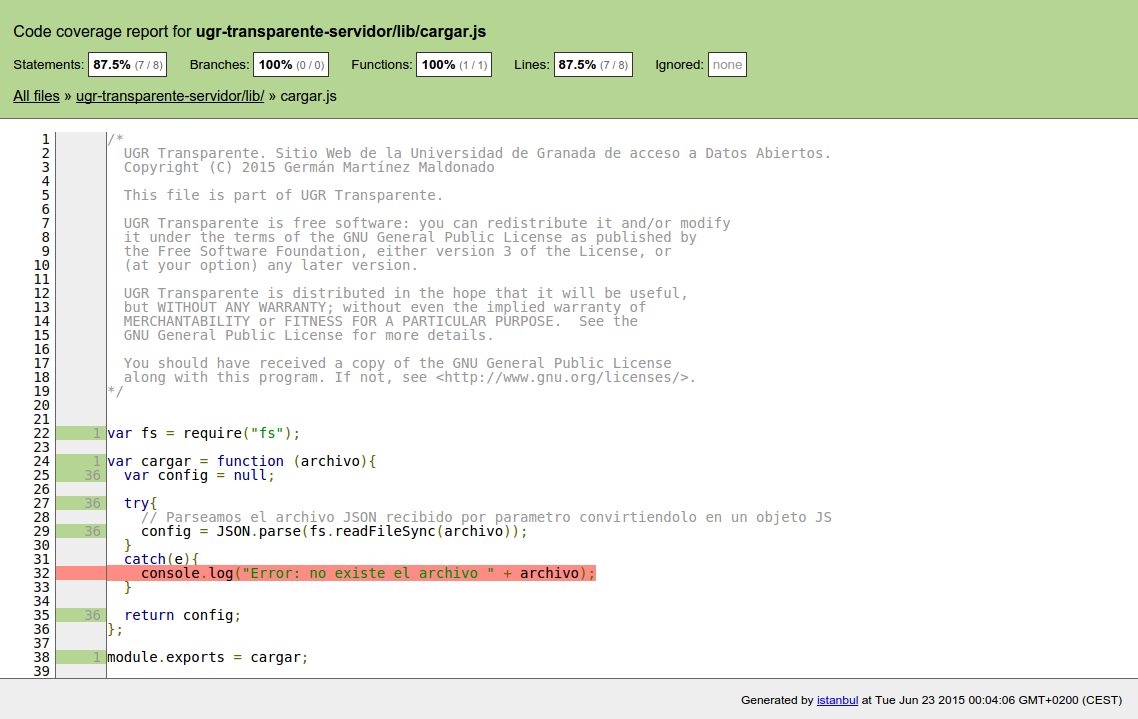
\includegraphics[width=1\textwidth]{../images/test_cobertura_03.png}
		\caption{}
		\label{fig:test_cobertura_03}
	\end{center}
\end{figure}

\section{Integración continua}

\begin{figure}[!ht]
	\begin{center}
		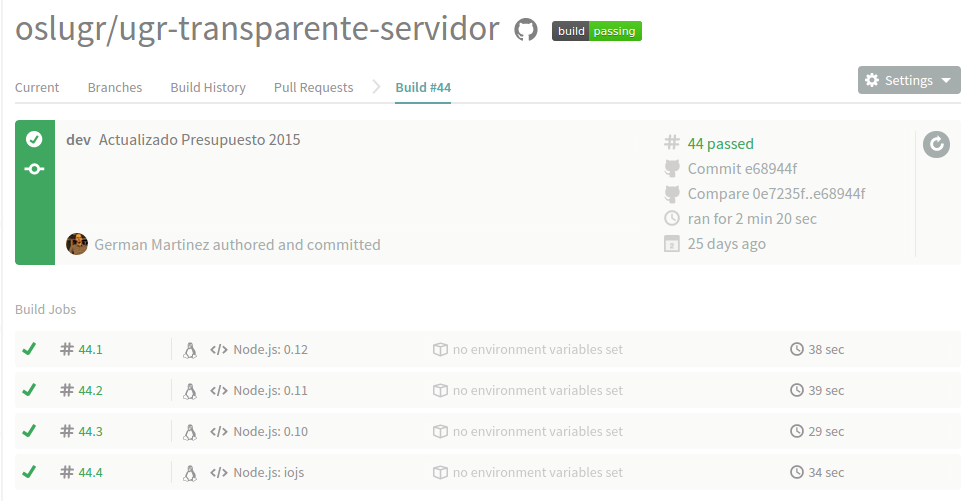
\includegraphics[width=1\textwidth]{../images/integracion_continua_01.png}
		\caption{}
		\label{fig:integracion_continua_01}
	\end{center}
\end{figure}

\begin{figure}[!ht]
	\begin{center}
		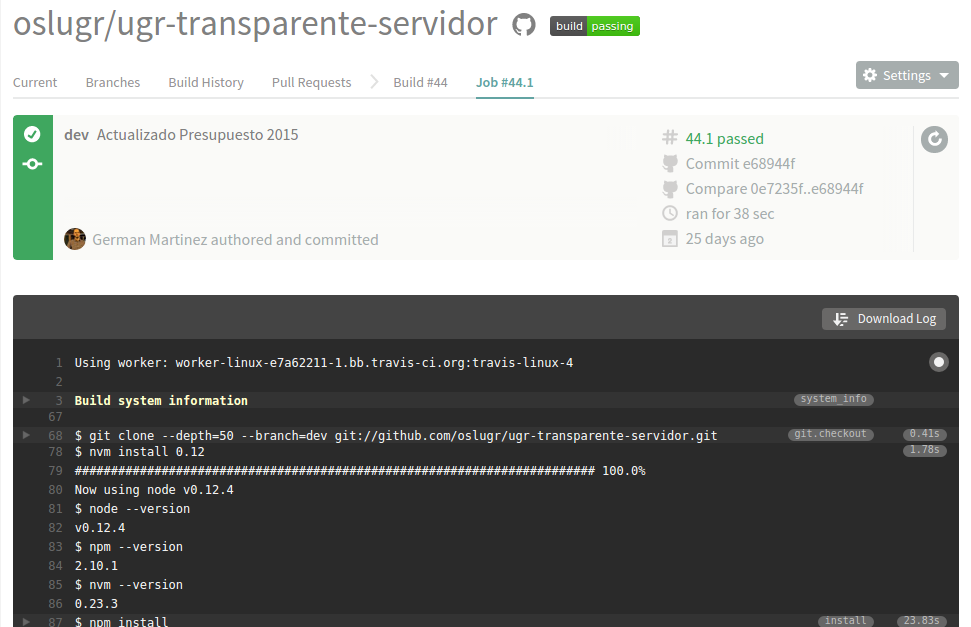
\includegraphics[width=1\textwidth]{../images/integracion_continua_02.png}
		\caption{}
		\label{fig:integracion_continua_02}
	\end{center}
\end{figure}

\begin{figure}[!ht]
	\begin{center}
		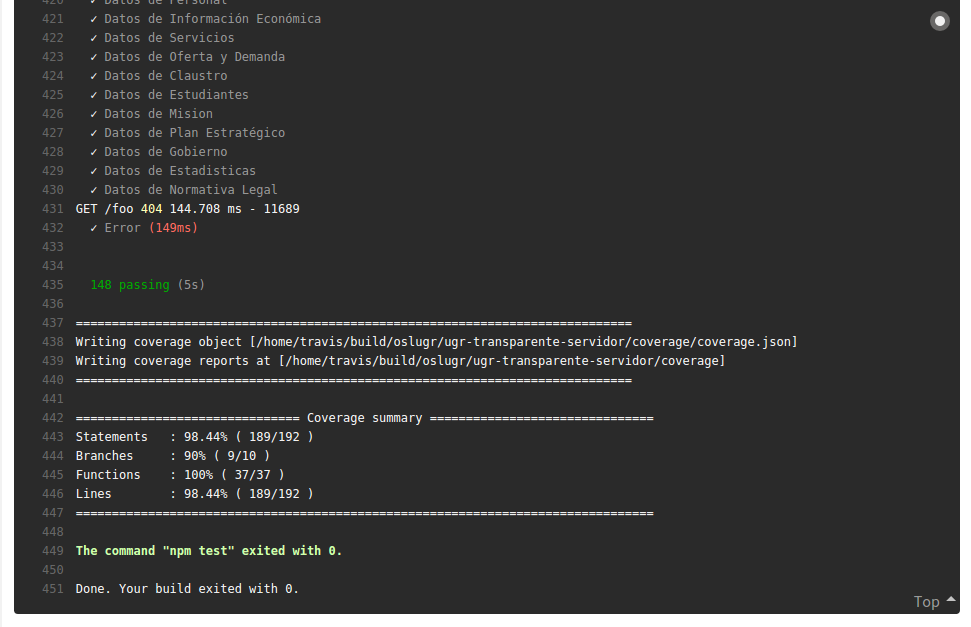
\includegraphics[width=1\textwidth]{../images/integracion_continua_03.png}
		\caption{}
		\label{fig:integracion_continua_03}
	\end{center}
\end{figure}

\newpage \
\newpage \
\newpage \
\newpage \
\newpage \
\section{Prueba de carga}

\subsection{Métricas y parámetros que afectan al rendimiento}

Para comparar las prestaciones de la aplicación debemos tener en cuenta los siguientes criterios:

\begin{itemize}
	\item El objetivo de esta prueba es medir las prestaciones del servidor generado por {\tt Express} para dar servicio a la aplicación del portal de transparencia bajo unas condiciones que nos aporte un análisis neutro del rendimiento del mismo.
	\item La herramienta que se usará para realizar estás mediciones es {\tt ApacheBench}.
	\item Los parámetros que se considerarán los parámetros usados en la herramienta: el número de peticiones que se realizan al servidor y el nivel de concurrencia con el que se realizan las peticiones.
	\item Los valores de estos parámetros irán modificándose para tener unos resultados más completos ante las diferentes cargas de trabajo que soportará el servidor.
\end{itemize}

El hardware y el software del sistema serán los siguientes:

\begin{itemize}
	\item \textbf{Hardware}:
	\begin{itemize}
		\item Procesador: Intel Pentium Dual CPU E2180 @ 2.00GHz
		\item Placa base: MSI MS-7255
		\item Chipset: VIA P4M900
		\item Memoria: 3GB (2+1 DIMM DDR2)
		\item Disco: Maxtor 6Y160P0 160GB 7200RPM
		\item Tarjeta gráfica: ATI Radeon X300SE 325MHz 128MB
		\item Red: Realtek RTL8100C 100Mbps
	\end{itemize}
	\item \textbf{Software}:
	\begin{itemize}
		\item Sistema operativo: Ubuntu 14.04.1 LTS i686 GNU/Linux
		\item Kernel: Linux 3.13.0-35-generic
		\item Sistema de archivos: ext4
	\end{itemize}
\end{itemize}

\subsection{Técnicas de evaluación, carga de trabajo y diseño de experimentos}

Para evaluar el rendimiento de la aplicación vamos a realizar benchmark hacia la aplicación en ejecución para poder realizar una evaluación sobre su comportamiento bajo diferentes cargas de trabajo. El programa con el que vamos hacer las pruebas es el ya mencionado {\tt ApacheBench}.
{\tt ApacheBench} es un aplicación en modo terminal que permite realizar de forma sencilla pruebas de rendimiento a cualquier servidor, sea cual sea el lenguaje en el que esté realizado. 

\bigskip
Según la información de registros de acceso del servidor en los últimos \textbf{6 meses} el número de peticiones de páginas del portal ha sido de \textbf{2.388 peticiones}, lo que sería aproximadamente \textbf{13 peticiones/día}. Para realizar los diferentes tests se realizará un \textbf{número de conexiones} variables al servidor (\textbf{30, 50 y 100}) con diferentes \textbf{niveles de concurrencia} en función del total de conexiones (\textbf{25\%, 50\% y 75\%}). Los números de conexiones para las prueba han sido elegidos para evaluar como se comportaría el servidor ante un gran aumento de actividad en el mismo en línea con el nivel de conexiones que se producen en la actualidad.

\bigskip
De entre las peticiones al portal, la página que ha recibido un mayor número de peticiones es la página de \textbf{Personal}, por lo que se van a realizar dos experimentos: el primero consistirá en realizar únicamente peticiones de la página de \textbf{Personal} a la aplicación; el segundo consistirá en realizar peticiones a distintas páginas de la aplicación de forma aleatorio. Estos experimentos nos permitirán comprobar como se comportará la aplicación en diferentes situaciones cono diferentes nivele de carga y la repercusión en su rendimiento ante estás diferentes pruebas, viendo por ejemplo si fuera necesario buscar una forma de balancear la carga del servidor. 

\bigskip
En total cada experimento constará de 9 pruebas, y a su vez cada una de estas pruebas se repetirá 10 veces consecutivas para así asegurarnos que los resultados son legítimos y no producto de sucesos fortuitos.

\bigskip
Las variables respuestas a tener en cuenta para el estudio serán:

\begin{itemize}
	\item Tiempo de ejecución.
	\item Solicitudes por segundo.
	\item Tiempo por solicitud concurrente.
	\item Velocidad de transferencia.
\end{itemize}

\bigskip
El único factor para los experimentos serán, como hemos dicho, el servidor de la aplicación desarrollada del portal de transparencia {\tt UGR Transparente}. Cuando se disponga de los resultados de todas las pruebas, se procederá a analizar e interpretar los resultados.

\subsection{Presentación de los resultados}

Enumeración de las pruebas a realizar por cada experimento:

\begin{itemize}
	\item \textbf{P1}: 30 solicitudes, concurrencia del 25\% (8).
	\item \textbf{P2}: 30 solicitudes, concurrencia del 50\% (15).
	\item \textbf{P3}: 30 solicitudes, concurrencia del 75\% (23).
	\item \textbf{P4}: 50 solicitudes, concurrencia del 25\% (13).
	\item \textbf{P5}: 50 solicitudes, concurrencia del 50\% (25).
	\item \textbf{P6}: 50 solicitudes, concurrencia del 75\% (38).
	\item \textbf{P7}: 100 solicitudes, concurrencia del 25\% (25).
	\item \textbf{P8}: 100 solicitudes, concurrencia del 50\% (50).
	\item \textbf{P9}: 100 solicitudes, concurrencia del 75\% (75).
\end{itemize}

\subsubsection{Experimento 1: peticiones a Personal}

\begin{itemize}
	\item \textbf{Tiempo de ejecución}
	\item \textbf{Solicitudes por segundo}
	\item \textbf{Tiempo por solicitud concurrente}
	\item \textbf{Velocidad de transparencia}
\end{itemize}